\documentclass[twocolumn]{article}
\usepackage{graphicx}
\usepackage{siunitx}
\usepackage{url}
\newcommand{\squared}{\textsuperscript{2}}
\date{1 September 2024}
\title{
\author{Joe Loughry and Kasper Rasmussen}
\begin{document}
\maketitle
\begin{abstract}
3000 word article for \emph{\texttt{.login}}
\end{abstract}
\section{Introduction}
What if you could do a glitching attack without access to the power supply?
What if you could do fault injection without boiling nitric acid, or grinding
wheels, and no longer limited to a microscope stage? The basilisk might be your
spirit animal.

With reference to the Black Hat USA talk mentioned earlier, the dog toy
represents a new kind of glitching attack, done through indicators rather than
the power supply.

Ours is more general than the usual glitching attack, which can only change the
return address; we can introduce our arbitrary code.

Glitching as usually introduced through the back door. We can extend to going
in through the front door.

If the eyes are the windows to the soul, LEDs are a window into the electronics.
\section{Detection of attack in progress}
Negative-going acknowledgement pulses, extending all the way ground
(Figure~\ref{figure:attack_signature}) are a distinctive signature indicating a
successful laser attack in progress on an I\squared C bus that is visible on an
oscilloscope \cite{Loughry2024c}. Their presence means that at least one
receiver on the I\squared C bus recognizes the laser as a legitimate sender and
has accepted a command from it.
\begin{figure}[ht]
  \centering
  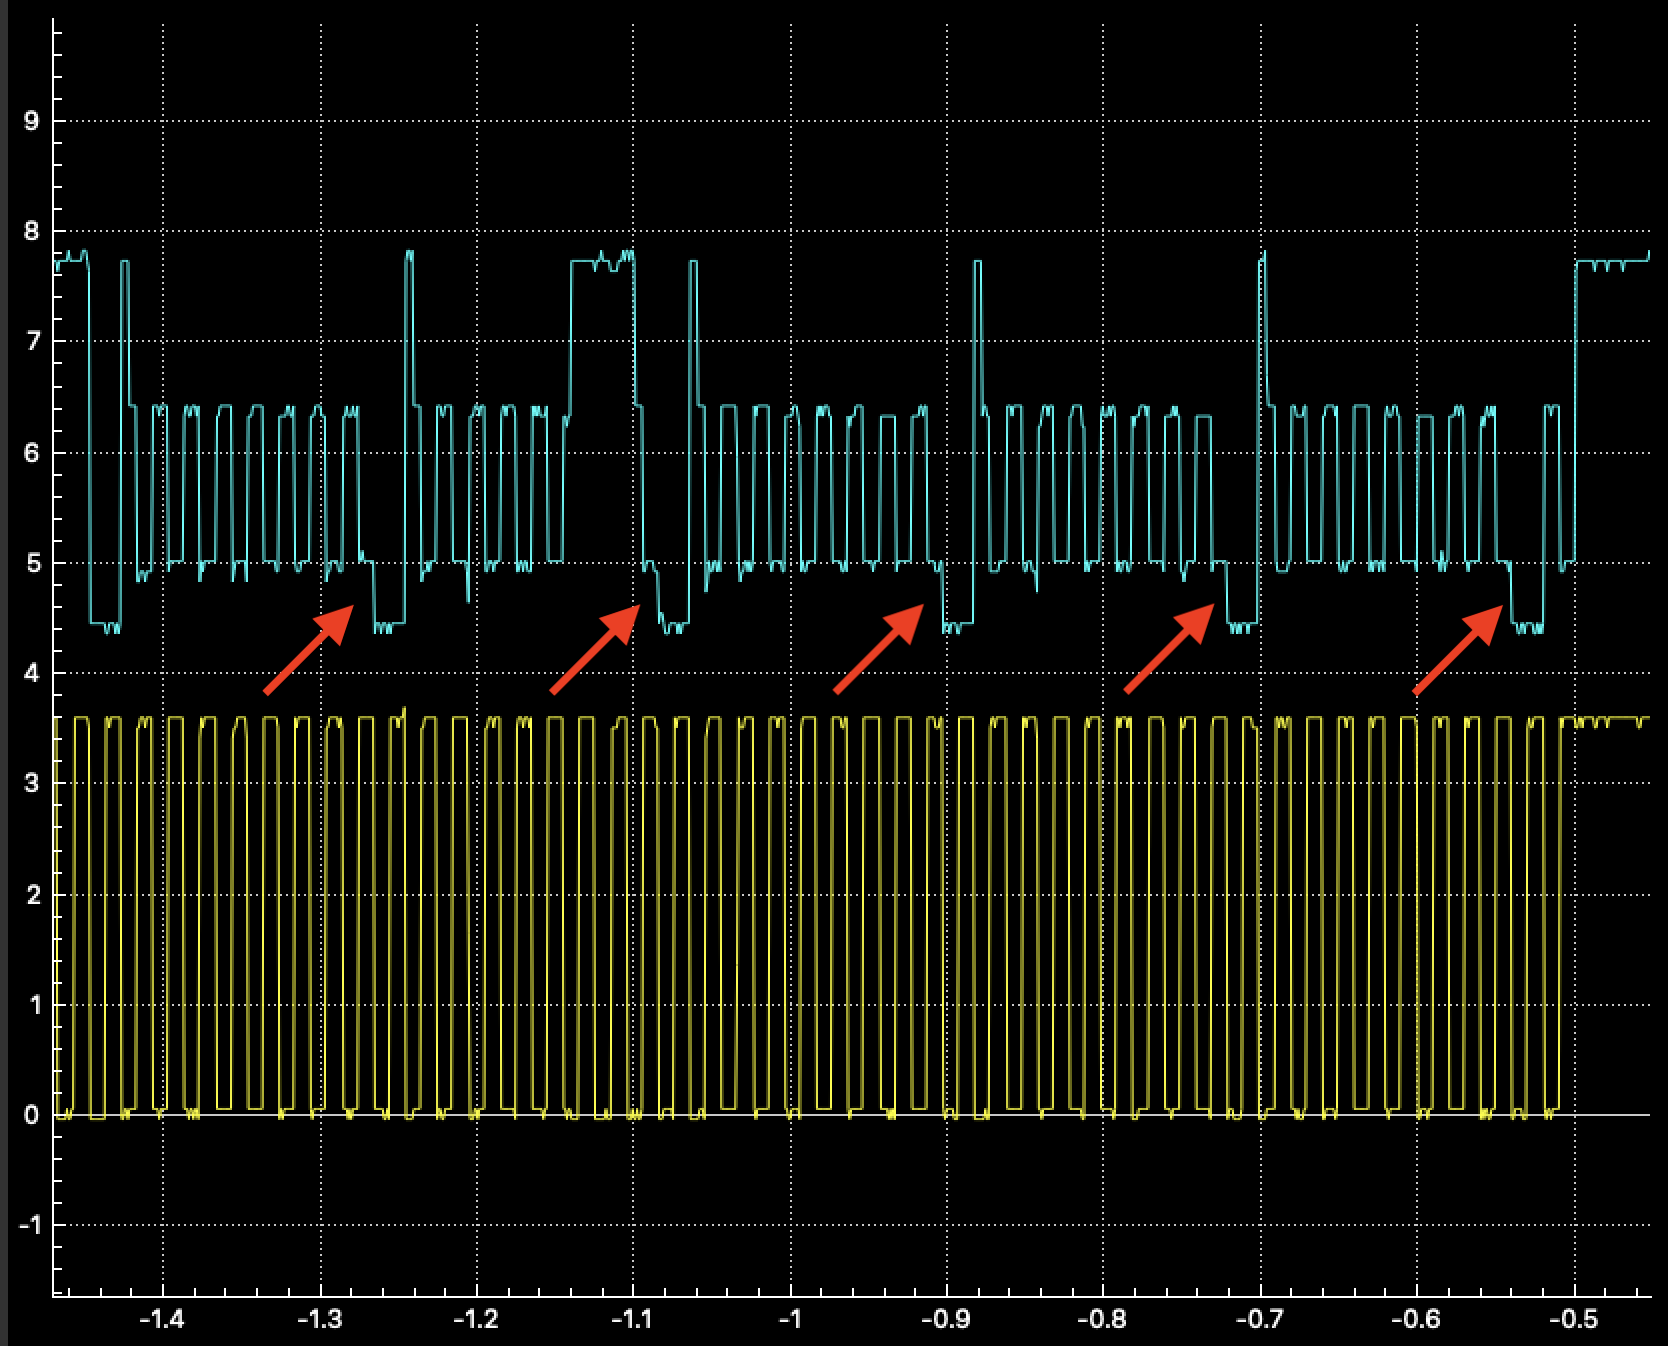
\includegraphics[width=\linewidth]{graphics/signature_of_the_attack.png}
  \caption{Negative-going acknowledgement pulses (red arrows) in the SDA signal
    are a distinctive signature of a successful photoconductive mode laser
    attack on an I\squared C bus.}
  \label{figure:attack_signature}
\end{figure}
\section{Summary and Conclusion}
What did we overlook? Show us what angles we missed.
\bibliographystyle{plain}
\bibliography{consolidated_bibtex_file}
\end{document}
